\section{Photo service}{Jose I. Retamal }
Jose I. Retamal
\vskip 0.1in
\indent
\indent
The photo-service provides image storage and access to them. It is composed of the main service, the database, and storage buckets.
The binary image is store as a public object in the bucket, and the URL to the image is stored in a MySQL database. Images can be accessed from the client using the public URL(
Figure \ref{photo:mainuml}). 

\begin{figure}[H]
	\begin{center}
		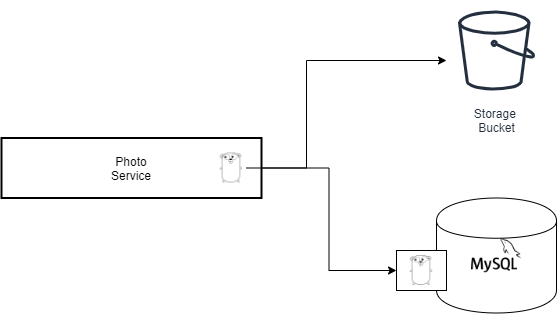
\includegraphics[width=120mm,scale=1]{img/photos/photos-main-uml.png}
		\caption{Authentication Service- UML.}
		\label{photo:mainuml}
	\end{center}
	
\end{figure}

\subsection{Request Sequence}

\subsubsection{Upload Image}

When the main service receives a request to upload an image, it generates a random URL, the image is upload to the bucket using that URL, and the URL is stored in the database. Then the URL is sent to the client for access to the image(figure \ref{photo:uploadsequence}).

\begin{figure}
	\begin{center}
		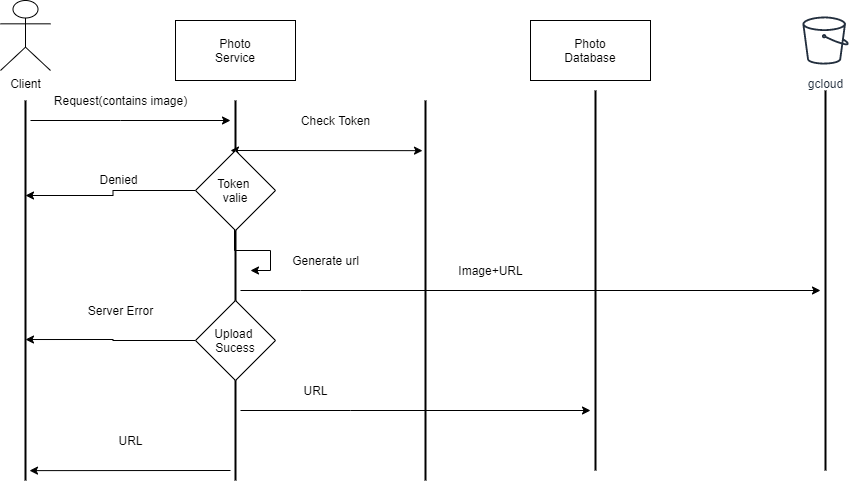
\includegraphics[width=90mm,scale=1]{img/photos/upload-image-sequence.png}
		\caption{Photo Service- upload Image Sequence Diagram.}
		\label{photo:uploadsequence}
	\end{center}
\end{figure}


\subsubsection{Get Image}

When the client requests an image, the client is first authenticated then the image URL is retrieved from the database. The URL is sent to the user who accesses the image directly from the bucket \ref{photo:getsequence}).

\begin{figure}
	\begin{center}
		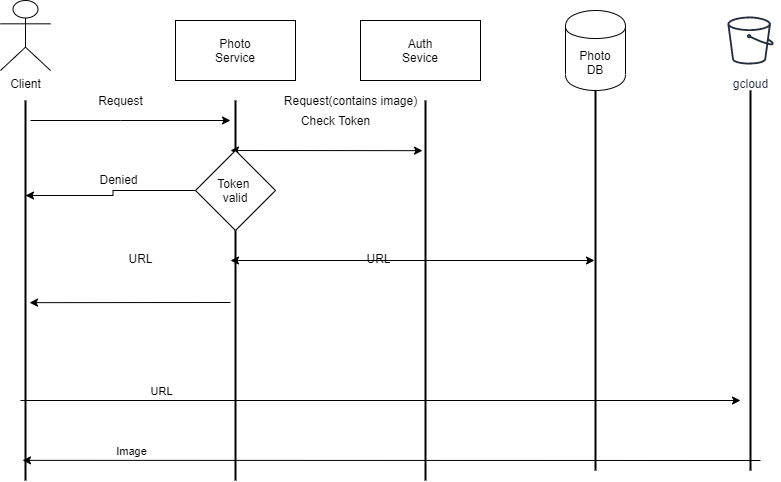
\includegraphics[width=90mm,scale=1]{img/photos/Image-request.png}
		\caption{Photo Service- Get Image Request Sequence Diagram.}
		\label{photo:getsequence}
	\end{center}
\end{figure}

\subsection{The Database}

The database store the URL to the image in the bucket. Images for City, Place, Posts, and User Profile are stored, there is a table for each of them(Figure \ref{photo:dbentity}).

All tables have an autogenerated integer primary key and each, and all images are also identified depending on the type. Bellow, we explain how they are linked using id from different databases.


\begin{figure}
	\begin{center}
		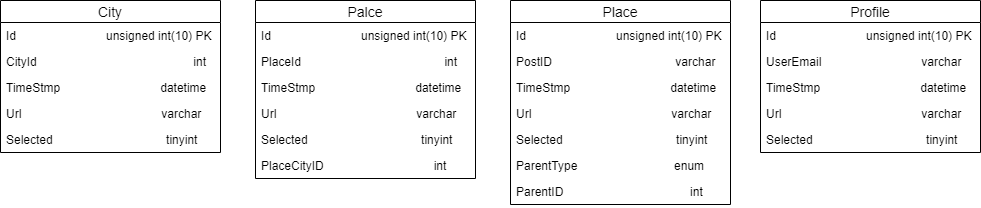
\includegraphics[width=90mm,scale=1]{img/photos/photo-db-entity.png}
		\caption{Photo Service-URLS Database Entity Diagram.}
		\label{photo:dbentity}
	\end{center}
\end{figure}

\begin{itemize}
	\item City Images
	
	\subitem The unique id is the CityId, which is the Neo4j unique id.
	
	\item	Place Images
	
	\subitem	The unique id is the PlaceId, which is the Neo4j unique id.
	
	\subitem The PlaceCityId is the id of the city of which the place belongs. It is used for getting all the images of the places in a city. 
	
	\item	PostImages
	
	\subitem The postId is the id of the post in MongoDB.
	
	\subitem There are two types of Posts, city and place post. They are stored in the same table, and an enum is used to distinguish.
	
	\item	Profile images
	
	\subitem The  UserEmail is the unique id, which is the PK in the auth database.
\end{itemize}

\subsection{The bucket}

Images are store in jpg format with a medium compression for maximum storage capacity without losing notable quality(Figure \ref{photo:buckerimage}).
Inside the bucket, images are public objects, and they can be accessed for anyone who has the URL. Folders organize objects (Figure \ref{photo:bucketfolder}), they are numbered, and more folders and buckets can be added.
The URL is generated randomly by the main service, which is composed of two integers for a fast generation of them.



\begin{figure}
	\begin{center}
		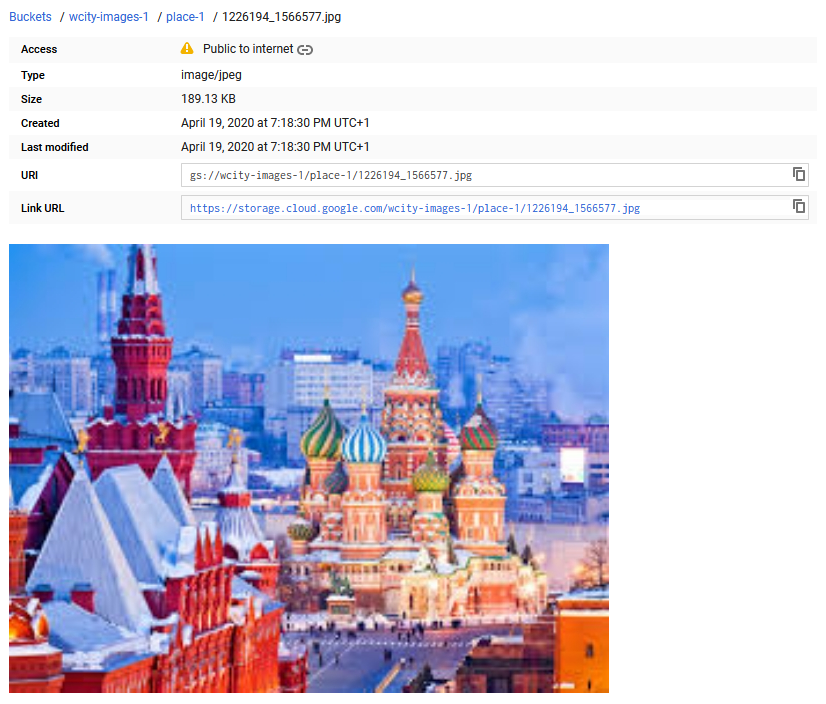
\includegraphics[width=90mm,scale=1]{img/photos/image-xample.png}
		\caption{Photo Service- Image in Bucker.}
		\label{photo:buckerimage}
	\end{center}
\end{figure}



\begin{figure}
	\begin{center}
		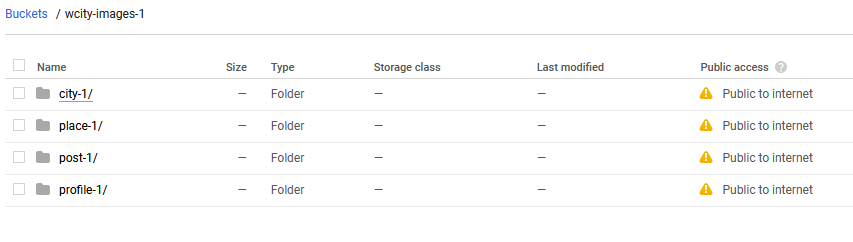
\includegraphics[width=90mm,scale=1]{img/photos/bucket-folders.png}
		\caption{Photo Service-Folders Structur in a Bucket.}
		\label{photo:bucketfolder}
	\end{center}
\end{figure}

